\documentclass[11pt,a4paper]{article}

\usepackage[margin=1in]{geometry}
\usepackage{amsmath,amssymb,amsthm,mathtools}
\usepackage{booktabs}
\usepackage{graphicx}
\usepackage{xcolor}
\usepackage{microtype}
\usepackage{enumitem}
\usepackage[hidelinks]{hyperref}

\newtheorem{theorem}{Theorem}[section]
\newtheorem{proposition}[theorem]{Proposition}
\newtheorem{lemma}[theorem]{Lemma}
\newtheorem{corollary}[theorem]{Corollary}
\theoremstyle{definition}
\newtheorem{definition}[theorem]{Definition}
\newtheorem{remark}[theorem]{Remark}

\DeclareMathOperator{\tr}{tr}
\DeclareMathOperator{\rank}{rank}
\DeclareMathOperator{\im}{im}
\DeclareMathOperator{\supp}{supp}
\DeclareMathOperator{\Gr}{Gr}
\DeclareMathOperator{\Var}{Var}
\newcommand{\C}{\mathbb{C}}
\newcommand{\R}{\mathbb{R}}
\newcommand{\Q}{\mathbb{Q}}
\newcommand{\ket}[1]{\lvert #1 \rangle}
\newcommand{\bra}[1]{\langle #1 \rvert}
\newcommand{\braket}[2]{\langle #1 \vert #2 \rangle}

\title{\textbf{Holomorphic Obstructions and Surrogate-Debiased Finite-Sample Spectral Certificates for Machine-Learned Quantum Monte Carlo}}
\author{Lluis Eriksson\thanks{Independent researcher (Sweden). Research, zero-dependency Lean~4 formalization, exact rational certificates, and reproducible benchmarks prepared with AI assistance (Google Antigravity) and publicly archived at \url{https://github.com/lluiseriksson/qcqmc-spectral-certificates}.}}
\date{November 24, 2026}

\begin{document}
\maketitle

\begin{abstract}
Recent hybrid quantum--classical quantum Monte Carlo (QC-QMC) workflows accelerate classical postprocessing of randomized quantum measurements by compressing noisy matchgate-shadow overlaps into differentiable machine-learning surrogates $f_\theta(\Phi)$ satisfying Slater-determinant equivariance $f_\theta(\Phi U) = \det(U) f_\theta(\Phi)$ (Jiang et al., \texttt{arXiv:2611.08151}, Nov.\ 2026). While this removes the $\mathcal{O}(N^3 N_s N_w N_\tau)$ shadow-evaluation bottleneck, it introduces two uncharacterized mathematical hazards: non-physical surrogate bias and uncertified statistical error. We resolve both with exact, machine-verified theory.
First, we give an elementary, self-contained Grassmannian characterization (Theorem~\ref{thm:holo}): for $1 \le \eta < N$, a $C^1$ $GL(\eta,\C)$-equivariant overlap surrogate represents a physical fermionic trial state $\ket{\Psi} \in \bigwedge^\eta \C^N$ if and only if $\bar{\partial} f_\theta \equiv 0$, equivalently if and only if the anti-holomorphic Green's defect $G^{\bar{\partial}}(\Phi)$ vanishes identically, equivalently if and only if $f_\theta$ annihilates all finite linear Slater-determinant syzygies (whereas for $\eta = N$ equivariance alone suffices). Left-projector affine backflow $G_0 + P_\Phi A$ collapses identically to a fixed Slater determinant (Remark~\ref{rem:collapse}), whereas general affine-trace or nonlinear backflow neural quantum surrogates (NQS) leave the physical Hilbert space, satisfy an exact sharp distance floor $\inf_{\ket{\Psi}} \|f_S - v_\Psi\|_2 = \|(I - S S^+) f_S^*\|_2$ (Theorem~\ref{thm:plucker}), and incur representation-dependent mixed-estimator bias even on zero-walker-error decompositions of the exact ground state $\ket{\Psi_0}$---including unphysical energies strictly below $E_0$ (Theorem~\ref{thm:bias}, demonstrated analytically and numerically on two-site Hubbard with zero error on computational-basis determinants yet $-0.971$ bias on rotated walkers).
Second, to turn noisy QC-QMC mixed overlap/energy data into rigorous spectral guarantees, we prove a sharp, universal \emph{Mixed-Energy Variational-Boost Law} (Theorem~\ref{thm:boost}): for any Hermitian $H \preceq E_{\max} I$ and unit states $(\ket{\Psi_{\mathrm{sur}}}, \ket{\Psi_T})$ with $|b_0| < 1$ and $E_{\mathrm{sur}} < E_{\max}$,
\[
  E_0 \;\le\; E_{\mathrm{sur}} - \frac{\lvert \bra{\Psi_{\mathrm{sur}}} (E_{\mathrm{sur}} I - H) \ket{\Psi_T} \rvert^2}{(E_{\max} - E_{\mathrm{sur}})(1 - |b_0|^2)},
\]
requiring neither measurement of $\bra{\Psi_T} H \ket{\Psi_T}$ nor variationality of the raw mixed energy. Generalizing to degree $d \ge 0$ yields \emph{Surrogate-Anchored Block Hausdorff Certificates} (Theorem~\ref{thm:hausdorff}) for both ground-state upper bounds and oracle-free two-edge visible spectral-gap exclusion using only classical moments $a_k$ and distribution-free Median-of-Means confidence boxes on linear shadow cross-moments $\operatorname{Re}(b_k)$, paired with Prediction-Powered Inference (PPI) walker debiasing (Proposition~\ref{prop:ppi}). All core algebraic, complex-vector projection, variational-boost, and complex spectral-measure conic-dual soundness theorems are formally verified in Lean~4.35.0 (zero \texttt{sorry}, zero custom axioms, zero external dependencies), and all numerical dual certificates on a 4-site Hubbard benchmark are independently verified in exact rational arithmetic ($\Q$) via symmetry-checked pivoted $LDL^\top$ factorization over explicit rational moment enclosures.
\end{abstract}

\section{Introduction and Positioning}

Quantum--classical hybrid quantum Monte Carlo (QC-QMC) \cite{huggins2022unbiasing,zhang2003quantum} uses a correlated quantum trial state $\ket{\Psi_T}$ prepared on quantum hardware to guide classical phaseless auxiliary-field QMC (AFQMC) walks over Slater determinants $\ket{\phi(\Phi)}$. Using Clifford matchgate classical shadows \cite{wan2023matchgate,huang2020predicting}, trial overlaps $f_T(\Phi) = \braket{\Psi_T}{\phi(\Phi)}$ can be estimated without interactive quantum--classical feedback, but re-evaluating shadows across $N_w$ walkers and $N_\tau$ imaginary-time steps scales as $\mathcal{O}(N^3 N_s N_w N_\tau)$. In a landmark advance, Jiang et al.\ \cite{jiang2026machine} compressed matchgate-shadow data into differentiable machine-learning surrogates $f_\theta(\Phi)$---specifically a backflow neural quantum surrogate (NQS) on the complex Grassmannian and a nonorthogonal configuration interaction (NOCI) surrogate---enabling chemically accurate 40-qubit hardware demonstrations on Google's Willow processor.

This paradigm shift raises two fundamental mathematical questions that are not addressed by empirical benchmarking alone:
\begin{enumerate}[leftmargin=1.5em]
  \item \textbf{Physical representability and mixed-estimator validity:} Jiang et al.\ \cite[Eq.~(S2.19)]{jiang2026machine} enforce Slater-determinant equivariance $f_\theta(\Phi U) = \det(U) f_\theta(\Phi)$ by passing the orthogonal projector $P_\Phi = \Phi(\Phi^\dagger \Phi)^{-1} \Phi^\dagger$ into a backflow network $G_\theta(P_\Phi)$. Does equivariance guarantee that $f_\theta$ represents a valid quantum trial state $\ket{\Psi} \in \bigwedge^\eta \C^N$? If not, what happens to the mixed energy estimator $E_{\mathrm{mix}}^\theta$, which is exact and unbiased for any physical trial state regardless of overlap accuracy when walkers sample $\ket{\Psi_0}$?
  \item \textbf{Finite-sample certified spectral bounds from linear quantum shadows:} Standard phaseless AFQMC with an ML surrogate has uncertified systematic bias (both phaseless and surrogate-induced) and is non-variational. Can one convert \emph{only} linear quantum-shadow cross-overlaps $\operatorname{Re}\bra{\Psi_{\mathrm{sur}}} T^k \ket{\Psi_T}$ anchored to a classical physical surrogate $\ket{\Psi_{\mathrm{sur}}}$ into non-asymptotic, distribution-free, independently checkable upper bounds on $E_0$ and oracle-free visible spectral-gap certificates---without assuming Gaussian noise or measuring quadratic quantum moments $c_k = \bra{\Psi_T} T^k \ket{\Psi_T}$?
\end{enumerate}

\paragraph{Literature positioning and explicit boundaries.}
Recent operator-algebraic SDP hierarchies establish certified bulk spectral-gap upper bounds \cite{xu2026bulk}, lower-gap qubit certificates \cite{rao2025convergent}, and Euclidean correlator bootstraps \cite{cho2025bootstrapping}, assuming exact operator relations or noiseless correlators. Conversely, finite-sample Wishart--Loewner Hausdorff certificates \cite{eriksson2026finitesample} handle unknown covariance under Gaussian random sketches $Z = \langle g, u\rangle\langle g, v\rangle$, explicitly noting as an open limitation that Gaussian sketches are not tied to an experimentally direct quantum shadow protocol. Our contribution bridges these lines while keeping all claims strictly bounded:
\begin{itemize}[leftmargin=1.5em]
  \item We do \emph{not} claim a general lower bound on the full Hamiltonian mass gap; our two-edge localizer certifies spectrum strictly inside $(\theta_1, \theta_2)$ for the spectral measure visible to $\operatorname{span}\{\ket{\Psi_{\mathrm{sur}}}, \ket{\Psi_T}\}$. By choosing $\theta_2 = \theta_{\mathrm{cert}}$ from a certified single-edge ground-state bound ($\lambda_0 > \theta_{\mathrm{cert}}$), the certified eigenvalue in $(\theta_1, \theta_{\mathrm{cert}})$ is provably distinct from the ground state without any oracle knowledge of $E_0$.
  \item We do \emph{not} claim that Backflow NQS fails empirically in all regimes of \cite{jiang2026machine}; rather, we establish the exact geometric mechanism (non-holomorphicity $\bar{\partial} f_\theta \neq 0$) by which equivariant backflow breaks mixed-estimator unbiasedness, provide sharp derivative-free and derivative-based witnesses ($\eta_{\mathrm{Pl}}$ and $G^{\bar{\partial}}$), and provide projection and PPI debiasing remedies.
  \item Our distribution-free finite-sample shadow benchmark simulates exact Born-rule global Haar (3-design) shadows on $\C\ket{0} \oplus \mathcal{H}_D$; extending the identical Median-of-Means confidence-box interface to Clifford matchgate shadows \cite{wan2023matchgate} simply replaces the exact complex-safe 3-design variance bound $4 a_{2k}$ with the matchgate shadow variance bound $\mathcal{O}(\sqrt{N}\log N)$.
\end{itemize}

\section{Holomorphic Obstructions on the Complex Grassmannian}

Let $1 \le \eta \le N$ be integers and let $\mathcal{M}_{N,\eta}^{\mathrm{full}} := \{\Phi \in \C^{N\times \eta} : \rank(\Phi) = \eta\}$. Each $\Phi = [\phi_1,\dots,\phi_\eta] \in \mathcal{M}_{N,\eta}^{\mathrm{full}}$ defines an unnormalized Slater determinant $\ket{\phi(\Phi)} := \phi_1 \wedge \cdots \wedge \phi_\eta \in \bigwedge^\eta \C^N$ whose components in the lexicographic computational basis $\{e_I : I \in \binom{[N]}{\eta}\}$ are the $\eta \times \eta$ minors $\det(\Phi_I)$. Consequently, for any physical trial state $\ket{\Psi} \in \bigwedge^\eta \C^N$, the overlap functional
\[
  f_\Psi(\Phi) := \braket{\Psi}{\phi(\Phi)} = \sum_{I \in \binom{[N]}{\eta}} \Psi_I^* \det(\Phi_I)
\]
is holomorphic in $\Phi$ and satisfies $GL(\eta, \C)$-equivariance:
\begin{equation}\label{eq:equivariance}
  f(\Phi U) = \det(U)\, f(\Phi) \qquad \forall\, \Phi \in \mathcal{M}_{N,\eta}^{\mathrm{full}},\; \forall\, U \in GL(\eta, \C).
\end{equation}
In \cite[Eq.~(S2.19)--(S2.22)]{jiang2026machine}, a backflow neural quantum surrogate takes the form
\begin{equation}\label{eq:backflow}
  f_\theta(\Phi) = \det\!\big[G_\theta(P_\Phi)^\dagger \Phi\big], \qquad P_\Phi := \Phi (\Phi^\dagger \Phi)^{-1} \Phi^\dagger \in \Gr(\eta, N),
\end{equation}
which enforces \eqref{eq:equivariance} because $P_{\Phi U} = P_\Phi$. Following \cite[Eq.~(S2.22)]{jiang2026machine}, on the nonvanishing locus $\{f \neq 0\}$ define the anti-holomorphic Green's defect matrix
\begin{equation}\label{eq:gdbar}
  G_{pq}^{\bar{\partial}}(\Phi) := -\frac{1}{f(\Phi)} \sum_{k=1}^{\eta} \frac{\partial f}{\partial \Phi^*_{pk}}(\Phi)\, \Phi^*_{qk}, \qquad 1 \le p,q \le N.
\end{equation}

\begin{theorem}[Holomorphic Characterization of Equivariant Overlap Surrogates]\label{thm:holo}
Let $1 \le \eta \le N$ and let $f : \mathcal{M}_{N,\eta}^{\mathrm{full}} \to \C$ satisfy \eqref{eq:equivariance}.
\begin{enumerate}[label=(\roman*),leftmargin=1.8em]
  \item \textbf{Full-filling boundary ($\eta = N$):} Without any regularity assumption, $f(\Phi) = f(I_N)\det(\Phi) = \braket{\Psi}{\phi(\Phi)}$ for the unique state $\ket{\Psi} = f(I_N)^* e_{[N]} \in \bigwedge^N \C^N$.
  \item \textbf{Nontrivial regime ($1 \le \eta < N$):} Assume $f \in C^1(\mathcal{M}_{N,\eta}^{\mathrm{full}}, \C)$. The following are equivalent:
  \begin{enumerate}[label=(\alph*),leftmargin=1.6em]
    \item \emph{Physical representability:} there exists a unique $\ket{\Psi} \in \bigwedge^\eta \C^N$ such that $f(\Phi) = \braket{\Psi}{\phi(\Phi)}$ for all $\Phi \in \mathcal{M}_{N,\eta}^{\mathrm{full}}$.
    \item \emph{Holomorphicity / vanishing Green's defect:} $\frac{\partial f}{\partial \Phi^*_{pk}}(\Phi) = 0$ for all $\Phi \in \mathcal{M}_{N,\eta}^{\mathrm{full}}$ and all $(p,k)$; equivalently, $G^{\bar{\partial}}(\Phi) = 0$ for all $\Phi$ with $f(\Phi) \neq 0$.
    \item \emph{Pl\"ucker linearity:} for every finite family $\{(\alpha_j, \Phi_j)\}_{j=1}^m$ satisfying $\sum_{j=1}^m \alpha_j \ket{\phi(\Phi_j)} = 0$ in $\bigwedge^\eta \C^N$, one has $\sum_{j=1}^m \alpha_j f(\Phi_j) = 0$.
  \end{enumerate}
  Moreover, the equivalence (a) $\Leftrightarrow$ (c) holds for arbitrary functions $f$ without $C^1$ regularity.
\end{enumerate}
\end{theorem}

\begin{proof}
Part (i) is immediate since $\mathcal{M}_{N,N}^{\mathrm{full}} = GL(N,\C)$, so $f(\Phi) = f(I_N \Phi) = \det(\Phi) f(I_N)$.

For Part (ii), (a) $\Rightarrow$ (b) and (a) $\Rightarrow$ (c) follow directly from multilinearity and holomorphicity of $\Phi \mapsto \sum_I \Psi_I^* \det(\Phi_I)$. For (c) $\Rightarrow$ (a), the computational basis determinants $\{e_I : I \in \binom{[N]}{\eta}\}$ belong to $\{\ket{\phi(\Phi)} : \Phi \in \mathcal{M}_{N,\eta}^{\mathrm{full}}\}$ and span $\bigwedge^\eta \C^N$; condition (c) states precisely that $\ket{\phi(\Phi)} \mapsto f(\Phi)$ extends unambiguously to a linear functional on $\bigwedge^\eta \C^N$, which equals $\braket{\Psi}{\cdot}$ for a unique $\ket{\Psi} \in \bigwedge^\eta \C^N$.

We next verify the internal equivalence in (b). Let $W(\Phi) \in \C^{N\times \eta}$ have entries $W_{pk} = \frac{\partial f}{\partial \Phi^*_{pk}}(\Phi)$, so $G^{\bar{\partial}}(\Phi) = -\frac{1}{f(\Phi)} W(\Phi)\Phi^\dagger$ on $U := \{f \neq 0\}$. Since $f \in C^1$ is continuous, $U$ is open. Because $\Phi$ has full column rank $\eta$, $\Phi^\dagger$ admits the right inverse $\Phi(\Phi^\dagger \Phi)^{-1}$, whence $G^{\bar{\partial}}(\Phi) = 0 \iff W(\Phi) = 0$ at every $\Phi \in U$. On $\operatorname{int}(U^c)$ we have $f \equiv 0$, so $W \equiv 0$ there as well. Since $U \cup \operatorname{int}(U^c)$ is open and dense in $\mathcal{M}_{N,\eta}^{\mathrm{full}}$ and $W$ is continuous, $G^{\bar{\partial}} \equiv 0$ on $U$ is equivalent to $W \equiv 0$ on all of $\mathcal{M}_{N,\eta}^{\mathrm{full}}$.

Finally, we give an elementary, self-contained proof of (b) $\Rightarrow$ (a) without invoking Hartogs extension or Borel--Weil--Bott. Fix $I_0 = \{1,\dots,\eta\}$ and partition $\Phi = \binom{A}{B}$ with $A \in \C^{\eta\times\eta}$ and $B \in \C^{(N-\eta)\times \eta}$. On the dense open chart $\mathcal{U}_{I_0} = \{\det A \neq 0\}$, equivariance \eqref{eq:equivariance} gives $f(\Phi) = \det(A)\, g_{I_0}(Z)$ with $Z := B A^{-1} \in \C^{(N-\eta)\times\eta}$ and $g_{I_0}(Z) := f\binom{I_\eta}{Z}$. Because $\binom{I_\eta}{Z} \in \mathcal{M}_{N,\eta}^{\mathrm{full}}$ for \emph{every} $Z \in \C^{(N-\eta)\times \eta}$, $g_{I_0}$ is entire on $\C^{(N-\eta)\times \eta}$; similarly $g_J$ is entire for every chart $J \in \binom{[N]}{\eta}$.
For any chart $J = (I_0 \setminus \{r\}) \cup \{\eta + s\}$ ($1 \le r \le \eta$, $1 \le s \le N-\eta$) and any $\Phi$ whose $I_0 \setminus \{r\}$ rows equal the standard basis rows $e_k^\top$ ($k \neq r$) and whose $(\eta + s)$-th row is $w^\top \in \C^{1\times\eta}$ with $w_r \neq 0$, permuting row $\eta + s$ into position $r$ via a permutation matrix $P$ gives $P A_J = I_\eta + e_r (w^\top - e_r^\top)$. Hence $\det A_J = \pm w_r$, and by the Sherman--Morrison formula,
\begin{equation}\label{eq:sherman_morrison}
  (P A_J)^{-1} = I_\eta + e_r \left(\frac{1 - w_r}{w_r}\, e_r^\top - \sum_{k \neq r} \frac{w_k}{w_r}\, e_k^\top\right),
\end{equation}
so row $r$ of $(P A_J)^{-1}$ equals $\frac{1}{w_r}\big(e_r^\top - \sum_{k \neq r} w_k e_k^\top\big)$ while every other row $k \neq r$ equals $e_k^\top$.

We apply \eqref{eq:sherman_morrison} to three families of affine lines $t \in \C$ (taking $|t| \to \infty$):
\begin{enumerate}[leftmargin=1.5em]
  \item \emph{Column-wise degree $\le 1$:} Fix $Z_0$, column $r$, and nonzero $z \in \C^{N-\eta}$, and set $Z(t) = Z_0 + t z e_r^\top$. Pick $s$ with $z_s \neq 0$ and $J = (I_0 \setminus \{r\}) \cup \{\eta + s\}$. On $\Phi(t) = \binom{I_\eta}{Z(t)}$, we have $w(t)_r = (Z_0)_{sr} + t z_s = \Theta(|t|)$ and $w(t)_k = (Z_0)_{sk}$ ($k \neq r$) constant in $t$. By \eqref{eq:sherman_morrison}, row $r$ of $(P A_J(t))^{-1}$ is $\mathcal{O}(|t|^{-1})$ while all other rows are $e_k^\top$. Because $t$ appears linearly only in column $r$ of the complementary block $B_J(t)$, the product $B_J(t) A_J(t)^{-1} = B_J(t) (P A_J(t))^{-1} P$ stays uniformly bounded as $|t| \to \infty$. Thus $|g_{I_0}(Z(t))| = |\det A_J(t)| \cdot |g_J(B_J(t) A_J(t)^{-1})| = \mathcal{O}(|t|)$, so by single-variable Liouville's theorem applied to $(g_{I_0}(Z(t)) - g_{I_0}(Z(0)))/t$, $g_{I_0}(Z(t))$ is affine in $t$.
  \item \emph{Row-wise degree $\le 1$:} Fix $Z_0$, row $s$, and nonzero $u \in \C^\eta$, and set $Z(t) = Z_0 + t e_s u^\top$. Pick $r$ with $u_r \neq 0$ and $J = (I_0 \setminus \{r\}) \cup \{\eta + s\}$. On $\Phi(t) = \binom{I_\eta}{Z(t)}$, $w(t)_k = (Z_0)_{sk} + t u_k$, so $\det A_J(t) = \pm((Z_0)_{sr} + t u_r) = \mathcal{O}(|t|)$, every entry of $(P A_J(t))^{-1}$ in \eqref{eq:sherman_morrison} is $\mathcal{O}(1)$, and $B_J(t)$ is completely independent of $t$. Hence $B_J(t) A_J(t)^{-1} = \mathcal{O}(1)$ and $|g_{I_0}(Z(t))| = \mathcal{O}(|t|)$, so $g_{I_0}(Z(t))$ is affine in $t$.
  \item \emph{Alternating symmetry:} If $\eta \ge 2$ and $N - \eta \ge 2$ (otherwise $g_{I_0}(Z)$ already has only one row or one column and is trivially a linear combination of $0\times 0$ and $1\times 1$ minors), take distinct rows $s_1 \neq s_2$ and distinct columns $r_1 \neq r_2$, and set $Z(t) = Z_0 + t(e_{s_1} + e_{s_2})(e_{r_1} + e_{r_2})^\top$. Multiply $\Phi(t) = \binom{I_\eta}{Z(t)}$ on the right by the unimodular matrix $U = I_\eta - E_{r_1, r_2}$ ($\det U = 1$), yielding $\widetilde{\Phi}(t) := \Phi(t) U = \binom{U}{Z(t) U}$ with $f(\widetilde{\Phi}(t)) = f(\Phi(t)) = g_{I_0}(Z(t))$. Crucially, column $r_2$ of $Z(t) U$ equals $(Z_0)_{:, r_2} - (Z_0)_{:, r_1}$ (independent of $t$), while $t$ appears linearly \emph{only} in column $r_1$ of $\widetilde{\Phi}(t)$ (in rows $\eta + s_1$ and $\eta + s_2$). Choose chart $J = (I_0 \setminus \{r_1\}) \cup \{\eta + s_1\}$ on $\widetilde{\Phi}(t)$: rows $k \in I_0 \setminus \{r_1\}$ of $U$ are still $e_k^\top$, and row $\eta + s_1$ has $w(t)_{r_1} = (Z_0)_{s_1, r_1} + t$ with all $w(t)_k$ ($k \neq r_1$) independent of $t$. By \eqref{eq:sherman_morrison}, $\det A_J(t) = \pm((Z_0)_{s_1, r_1} + t) = \mathcal{O}(|t|)$, row $r_1$ of $(P A_J(t))^{-1}$ decays as $\mathcal{O}(|t|^{-1})$, and all other rows are $e_k^\top$. Since $t$ appears linearly only in column $r_1$ of $B_J(t)$ (specifically at row $\eta + s_2$, while row $r_1$ of $U$ is the constant $e_{r_1}^\top - e_{r_2}^\top$), $B_J(t) A_J(t)^{-1}$ stays uniformly bounded as $|t| \to \infty$. Therefore $|g_{I_0}(Z(t))| = |f(\widetilde{\Phi}(t))| = |\det A_J(t)| \cdot |g_J(B_J(t) A_J(t)^{-1})| = \mathcal{O}(|t|)$, so $t \mapsto g_{I_0}(Z(t))$ has degree $\le 1$.
\end{enumerate}
Since $g_{I_0}$ is a polynomial of degree $\le 1$ in each row and column (by (1)--(2)), its $t^2$ coefficient along $Z(t)$ in (3) is the sum of the coefficients of $Z_{s_1, r_1} Z_{s_2, r_2}$ and $Z_{s_1, r_2} Z_{s_2, r_1}$ (multiplying any monomial in the remaining rows and columns), which must therefore vanish identically. Thus $g_{I_0}(Z)$ is alternating under transposition of any pair of rows or columns and is an exact linear combination of minors of $Z$. By Jacobi's complementary minor identity, $\det(A) \cdot \det((B A^{-1})_{S,R}) = \pm \det(\Phi_{(I_0\setminus R)\cup(\eta+S)})$, so $f(\Phi) = \sum_{K \in \binom{[N]}{\eta}} c_K \det(\Phi_K)$ on the dense open set $\mathcal{U}_{I_0}$, and by continuity on all of $\mathcal{M}_{N,\eta}^{\mathrm{full}}$.
\end{proof}

\begin{remark}[Two-Spin Product Extension]
For $C^1$ spin-separated surrogates $f(\Phi_\alpha, \Phi_\beta)$ on $\mathcal{M}_{N,\eta_\alpha}^{\mathrm{full}} \times \mathcal{M}_{N,\eta_\beta}^{\mathrm{full}}$ ($1 \le \eta_\alpha, \eta_\beta \le N$) equivariant under $GL(\eta_\alpha,\C)\times GL(\eta_\beta,\C)$ as in \cite[Eq.~(S2.19)]{jiang2026machine}, applying Theorem~\ref{thm:holo} (Part (i) if $\eta_\sigma = N$, Part (ii) if $\eta_\sigma < N$) first to $\Phi_\alpha$ at fixed $\Phi_\beta$ and then to each resulting holomorphic $GL(\eta_\beta)$-equivariant minor coefficient $f(E_I, \Phi_\beta)$ yields the identical characterization: $f(\Phi_\alpha,\Phi_\beta) = \braket{\Psi}{\phi(\Phi_\alpha)\otimes\phi(\Phi_\beta)}$ for a unique $\ket{\Psi} \in \bigwedge^{\eta_\alpha}\C^N \otimes \bigwedge^{\eta_\beta}\C^N$ if and only if $\partial f / \partial \Phi_\alpha^* \equiv 0$ and $\partial f / \partial \Phi_\beta^* \equiv 0$.
\end{remark}

\begin{remark}[Left-Projector Collapse vs.\ Non-Holomorphic Affine/Nonlinear Backflow]\label{rem:collapse}
Not every non-constant orbital map $G_\theta(P_\Phi)$ produces a non-holomorphic surrogate. If $G_\theta(P_\Phi) = G_0 + P_\Phi A$ is \emph{left-projector affine} in $P_\Phi$, then since $P_\Phi^\dagger = P_\Phi$ and $P_\Phi \Phi = \Phi$,
\[
  G_\theta(P_\Phi)^\dagger \Phi = G_0^\dagger \Phi + A^\dagger P_\Phi \Phi = (G_0 + A)^\dagger \Phi,
\]
so $f_\theta$ collapses identically to the single fixed Slater determinant $\det[(G_0 + A)^\dagger \Phi]$ and is secretly holomorphic. Conversely, general affine maps in $P_\Phi$ that couple across orbitals via left multipliers or scalar traces---such as $G_0 + B P_\Phi A$ (when $B$ does not commute with $P_\Phi$) or $G_0 + \kappa \tr(M_{\mathrm{obs}} P_\Phi) A_{\mathrm{bf}}$ (Experiment~1 below)---as well as nonlinear backflow networks in $P_\Phi$ evade this collapse precisely by introducing genuine $\Phi^*$-dependence, which generically breaks $\bar{\partial} f_\theta = 0$.
\end{remark}

\subsection{Exact Distance-to-Physical-States Witness and Mixed-Estimator Bias}

\begin{theorem}[Pl\"ucker-Kernel Distance Floor and Holomorphic Projection Restoration]\label{thm:plucker}
Let $\{\Phi_1,\dots,\Phi_m\} \subset \mathcal{M}_{N,\eta}^{\mathrm{full}}$ be any finite set of (possibly complex) walkers, let $W \in \C^{D \times m}$ ($D = \binom{N}{\eta}$) have columns $\ket{\phi(\Phi_a)}$, and let $S := W^\dagger W \in \C^{m\times m}$ be their exact overlap Gram matrix with Moore--Penrose pseudoinverse $S^+$. For any overlap surrogate $f$ with evaluation vector $f_S := (f(\Phi_1),\dots,f(\Phi_m))^\top \in \C^m$, define the \emph{Pl\"ucker-kernel witness}
\begin{equation}\label{eq:eta_pl}
  \eta_{\mathrm{Pl}}(f; S) := \big\|(I_m - S S^+) f_S^*\big\|_2 = \big\|(I_m - S^\top (S^\top)^+) f_S\big\|_2.
\end{equation}
Then for every physical trial state $\ket{\Psi} \in \bigwedge^\eta \C^N$ with overlap vector $(v_\Psi)_a := \braket{\Psi}{\phi(\Phi_a)}$,
\[
  \inf_{\ket{\Psi} \in \bigwedge^\eta \C^N} \|f_S - v_\Psi\|_2 \;=\; \eta_{\mathrm{Pl}}(f; S),
\]
and the infimum is uniquely attained within $\mathcal{V}_m := \operatorname{span}\{\ket{\phi(\Phi_a)}\}$ by the holomorphic projection
\begin{equation}\label{eq:proj_state}
  \ket{\Psi_f^{\mathrm{proj}}} := W S^+ f_S^* \;=\; \sum_{a,b=1}^m (S^+)_{ab}\, f(\Phi_b)^*\, \ket{\phi(\Phi_a)}.
\end{equation}
In particular, for any Hermitian Hamiltonian $H$ on $\bigwedge^\eta \C^N$ with ground-state energy $E_0 = \lambda_{\min}(H)$, whenever $\ket{\Psi_f^{\mathrm{proj}}} \neq 0$, its Rayleigh quotient $E_{\mathrm{var}}(f;S) := \frac{\bra{\Psi_f^{\mathrm{proj}}} H \ket{\Psi_f^{\mathrm{proj}}}}{\braket{\Psi_f^{\mathrm{proj}}}{\Psi_f^{\mathrm{proj}}}} \ge E_0$ is a strict variational upper bound on $E_0$.
\end{theorem}

\begin{proof}
For any $\ket{\Psi} \in \C^D$, $(v_\Psi)_a = \braket{\Psi}{\phi(\Phi_a)} = (W^\dagger \Psi)_a^*$, so $\|f_S - v_\Psi\|_2 = \|f_S^* - W^\dagger \Psi\|_2$. Because $\im(W^\dagger) = \im(W^\dagger W) = \im(S)$, the orthogonal projector onto $\im(W^\dagger)$ is $\Pi_S := S S^+$. Decomposing $f_S^* = \Pi_S f_S^* + (I_m - \Pi_S) f_S^*$, orthogonality gives
\[
  \|f_S^* - W^\dagger \Psi\|_2^2 = \|(I_m - S S^+) f_S^*\|_2^2 + \|S S^+ f_S^* - W^\dagger \Psi\|_2^2 \ge \eta_{\mathrm{Pl}}(f; S)^2.
\]
Setting $\ket{\Psi_f^{\mathrm{proj}}} = W S^+ f_S^*$ yields $W^\dagger \Psi_f^{\mathrm{proj}} = S S^+ f_S^*$, attaining exact equality; uniqueness inside $\mathcal{V}_m = \im(W) = \ker(W^\dagger)^\perp$ holds because any two minimizers differ in $\ker(W^\dagger) \cap \mathcal{V}_m = \{0\}$. Note the complex conjugation $f_S^*$: for complex walkers (standard in AFQMC due to complex Hubbard--Stratonovich fields), $v_\Psi \in \im(S^\top) = \im(S^*)$, whereas $v_\Psi^* \in \im(S)$.
\end{proof}

Now consider a factorized fermionic Hamiltonian $H = E_{\mathrm{core}} + \hat{B}_0 + \sum_\gamma c_\gamma \hat{B}_\gamma^2$ with Hermitian one-body matrices $B_0, B_\gamma$ and $c_\gamma \in \R$ \cite[Eq.~(S2.9)]{jiang2026machine}. Following \cite[Eq.~(S2.21)]{jiang2026machine}, define the Lie-derivative operators $\mathcal{D}_B[f](\Phi) := -i \partial_s f(e^{isB}\Phi)|_{s=0}$, $\mathcal{D}_B^2[f](\Phi) := -\partial_s^2 f(e^{isB}\Phi)|_{s=0}$, and the surrogate local-energy numerator
\[
  \mathcal{L}_H[f](\Phi) := E_{\mathrm{core}} f(\Phi) + \mathcal{D}_{B_0}[f](\Phi) + \sum_\gamma c_\gamma \mathcal{D}_{B_\gamma}^2[f](\Phi), \qquad E_L^f(\Phi) := \frac{\mathcal{L}_H[f](\Phi)}{f(\Phi)}.
\]
By the chain rule, $\mathcal{D}_B[f](\Phi) = \sum_{p,k}\frac{\partial f}{\partial \Phi_{pk}}(B\Phi)_{pk} - \sum_{p,k}\frac{\partial f}{\partial \Phi^*_{pk}}(B\Phi)^*_{pk}$, reproducing \cite[Eq.~(S2.22)]{jiang2026machine}. For any physical state $f_\Psi$, $\mathcal{L}_H[f_\Psi](\Phi) = \bra{\Psi} H \ket{\phi(\Phi)}$.

\begin{theorem}[Exact Mixed-Estimator Bias Decomposition]\label{thm:bias}
Let $f = f_\Psi + r$ be any decomposition of a $C^2$ equivariant surrogate into a physical state overlap $f_\Psi$ and a non-holomorphic residual $r$. For any finite walker ensemble $\{(w_i, \Phi_i)\}_{i=1}^{N_w}$ with $f(\Phi_i) \neq 0$, total weight $W_{\mathrm{tot}} := \sum_{i=1}^{N_w} w_i \neq 0$, and represented state $\ket{\widetilde{\Psi}} := \sum_{i=1}^{N_w} \frac{w_i}{f(\Phi_i)} \ket{\phi(\Phi_i)}$, the mixed energy estimator $E_{\mathrm{mix}}^f := \frac{1}{W_{\mathrm{tot}}} \sum_{i=1}^{N_w} w_i E_L^f(\Phi_i)$ satisfies
\begin{equation}\label{eq:bias_decomp}
  E_{\mathrm{mix}}^f - E_0 \;=\; \frac{\bra{\Psi}(H - E_0)\ket{\widetilde{\Psi}}}{W_{\mathrm{tot}}} \;+\; \frac{1}{W_{\mathrm{tot}}} \sum_{i=1}^{N_w} \frac{w_i}{f(\Phi_i)} \big(\mathcal{L}_H[r](\Phi_i) - E_0 r(\Phi_i)\big).
\end{equation}
Consequently, even on a \emph{zero-walker-error} ensemble representing the exact ground state ($\ket{\widetilde{\Psi}} = \ket{\Psi_0}$), the first term vanishes identically while the second term leaves a generically nonzero, representation-dependent non-holomorphic bias.
\end{theorem}

\begin{proof}
Using $W_{\mathrm{tot}} = \sum_i \frac{w_i}{f(\Phi_i)} f(\Phi_i)$ and linearity of $\mathcal{L}_H$,
\begin{align*}
  W_{\mathrm{tot}}(E_{\mathrm{mix}}^f - E_0)
  &= \sum_{i=1}^{N_w} \frac{w_i}{f(\Phi_i)}\big(\mathcal{L}_H[f](\Phi_i) - E_0 f(\Phi_i)\big) \\
  &= \sum_{i=1}^{N_w} \frac{w_i}{f(\Phi_i)}\big(\mathcal{L}_H[f_\Psi](\Phi_i) - E_0 f_\Psi(\Phi_i)\big)
   + \sum_{i=1}^{N_w} \frac{w_i}{f(\Phi_i)}\big(\mathcal{L}_H[r](\Phi_i) - E_0 r(\Phi_i)\big).
\end{align*}
Since $\mathcal{L}_H[f_\Psi](\Phi_i) - E_0 f_\Psi(\Phi_i) = \bra{\Psi}(H - E_0)\ket{\phi(\Phi_i)}$, linearity of $\bra{\Psi}(H - E_0)\ket{\cdot}$ collapses the first sum to $\bra{\Psi}(H - E_0)\ket{\widetilde{\Psi}}$. Dividing by $W_{\mathrm{tot}}$ gives \eqref{eq:bias_decomp}.
\end{proof}

\section{Universal Mixed-Energy Variational-Boost Law}

Because raw mixed energies $E_{\mathrm{mix}} = \frac{\bra{\Psi_{\mathrm{sur}}} H \ket{\Psi_T}}{\braket{\Psi_{\mathrm{sur}}}{\Psi_T}}$ are non-variational (and can be complex when $\ket{\Psi_T}$ is not an eigenstate), QC-QMC normally cannot certify $E_0$ from mixed overlaps alone. The following universal, sharp inequality resolves this directly; it may be viewed as a $2\times 2$ Schur-complement upper-bound counterpart to Temple's lower-bound inequality, replacing second-moment $H^2$ data with linear mixed residuals $d_H$ and an upper spectral enclosure $E_{\max}$.

\begin{theorem}[Universal Mixed-Energy Variational-Boost Law]\label{thm:boost}
Let $H$ be any Hermitian operator on a finite-dimensional Hilbert space satisfying $H \preceq E_{\max} I$ with ground-state energy $E_0 = \lambda_{\min}(H)$. Let $\ket{\Psi_{\mathrm{sur}}}, \ket{\Psi_T}$ be unit vectors with overlap $b_0 := \braket{\Psi_{\mathrm{sur}}}{\Psi_T}$ satisfying $|b_0| < 1$, classical surrogate energy $E_{\mathrm{sur}} := \bra{\Psi_{\mathrm{sur}}} H \ket{\Psi_{\mathrm{sur}}} < E_{\max}$, and linear mixed energy residual $d_H := \bra{\Psi_{\mathrm{sur}}} (E_{\mathrm{sur}} I - H) \ket{\Psi_T}$ ($= b_0(E_{\mathrm{sur}} - E_{\mathrm{mix}})$ when $b_0 \neq 0$). Then
\begin{equation}\label{eq:boost}
  E_0 \;\le\; E_{\mathrm{sur}} - \frac{|d_H|^2}{(E_{\max} - E_{\mathrm{sur}})(1 - |b_0|^2)}.
\end{equation}
Inequality \eqref{eq:boost} holds unconditionally (including for $b_0 = 0$, complex $E_{\mathrm{mix}}$, and $E_{\mathrm{mix}} > E_{\mathrm{sur}}$) and is sharp: letting $A := E_{\max} I - H$, $\mathcal{S} := \operatorname{span}\{\ket{\Psi_{\mathrm{sur}}}, \ket{\Psi_T}\}$, and $A|_{\mathcal{S}} := P_{\mathcal{S}} A P_{\mathcal{S}}$ be the $2\times 2$ compression of $A$ to $\mathcal{S}$, equality holds for $d_H \neq 0$ if and only if $\rank(A|_{\mathcal{S}}) = 1$ and $\lambda_{\max}(A|_{\mathcal{S}}) = E_{\max} - E_0$ (equivalently, $\mathcal{S} = \operatorname{span}\{\ket{\Psi_0}, \ket{\Psi_{\max}}\}$ with $H\ket{\Psi_0} = E_0\ket{\Psi_0}$ and $H\ket{\Psi_{\max}} = E_{\max}\ket{\Psi_{\max}}$), and for $d_H = 0$ if and only if $E_{\mathrm{sur}} = E_0$.
\end{theorem}

\begin{proof}
Set $A := E_{\max} I - H \succeq 0$ and $\lambda := \lambda_{\max}(A) = E_{\max} - E_0$. Decompose $\ket{\Psi_T} = b_0 \ket{\Psi_{\mathrm{sur}}} + \sqrt{1 - |b_0|^2}\,\ket{w}$ with $\braket{\Psi_{\mathrm{sur}}}{w} = 0$ and $\|w\|_2 = 1$. Restricting $A$ to $\mathcal{S} = \operatorname{span}\{\ket{\Psi_{\mathrm{sur}}}, \ket{w}\}$ produces the $2\times 2$ positive semidefinite matrix
\[
  M = \begin{pmatrix} \alpha & \beta \\ \beta^* & \gamma \end{pmatrix} \succeq 0, \quad
  \alpha := \bra{\Psi_{\mathrm{sur}}} A \ket{\Psi_{\mathrm{sur}}} = E_{\max} - E_{\mathrm{sur}} > 0, \quad
  |\beta| = |\bra{\Psi_{\mathrm{sur}}} A \ket{w}| = \frac{|d_H|}{\sqrt{1 - |b_0|^2}},
\]
where $\gamma := \bra{w} A \ket{w}$ satisfies $M \succeq 0 \implies \alpha\gamma \ge |\beta|^2$ and $\lambda I_2 - M \succeq 0 \implies \lambda \ge \alpha$, $\lambda \ge \gamma$, and $(\lambda - \alpha)(\lambda - \gamma) \ge |\beta|^2$.
Suppose for contradiction that $\lambda < \alpha + |\beta|^2 / \alpha$. Then $0 \le \lambda - \alpha < |\beta|^2/\alpha$ (which forces $|\beta|^2/\alpha > 0$) and, since $\gamma \ge |\beta|^2/\alpha$, $0 \le \lambda - \gamma \le \lambda - |\beta|^2/\alpha < \alpha$. Multiplying these nonnegative inequalities gives $(\lambda - \alpha)(\lambda - \gamma) < (|\beta|^2/\alpha)\cdot \alpha = |\beta|^2$, contradicting $(\lambda - \alpha)(\lambda - \gamma) \ge |\beta|^2$. Hence $E_{\max} - E_0 = \lambda \ge \lambda_{\max}(M) \ge \alpha + |\beta|^2/\alpha$, which rearranges to \eqref{eq:boost}.
For sharpness when $d_H \neq 0$ ($\beta \neq 0$), equality requires both $\lambda = \lambda_{\max}(M)$ and $\lambda_{\max}(M) = \alpha + |\beta|^2/\alpha$; evaluating $\det((\alpha + |\beta|^2/\alpha) I_2 - M) = (|\beta|^2/\alpha)(|\beta|^2/\alpha - \gamma) \le 0$ shows the latter holds if and only if $\gamma = |\beta|^2/\alpha$, i.e., $\rank(M) = 1$, and then the unit eigenvector of $M$ with eigenvalue $\lambda$ is a ground state of $H$ while its orthogonal complement in $\mathcal{S}$ lies in $\ker(A) = \ker(E_{\max} I - H)$.
\end{proof}

\section{Surrogate-Anchored Block Hausdorff Certificates and Quantum Shadow Protocol}

Theorem~\ref{thm:boost} is the degree-$0$ instance of a full semidefinite moment hierarchy anchored to a classical physical surrogate $\ket{\Psi_{\mathrm{sur}}}$. Given an oracle-free spectral enclosure $E_{\min}^{\mathrm{box}} I \preceq H \preceq E_{\max}^{\mathrm{box}} I$ (e.g., via Gershgorin's theorem), define the rescaled contraction $T := (E_{\max}^{\mathrm{box}} I - H)/(E_{\max}^{\mathrm{box}} - E_{\min}^{\mathrm{box}}) \in [0, I]$ and the $2\times 2$ block Hausdorff moment sequence \cite{schmudgen2017moment}
\[
  B_k := \begin{pmatrix} a_k & b_k \\ b_k^* & c_k \end{pmatrix}
  := \begin{pmatrix} \bra{\Psi_{\mathrm{sur}}} T^k \ket{\Psi_{\mathrm{sur}}} & \bra{\Psi_{\mathrm{sur}}} T^k \ket{\Psi_T} \\ \bra{\Psi_T} T^k \ket{\Psi_{\mathrm{sur}}} & \bra{\Psi_T} T^k \ket{\Psi_T} \end{pmatrix}, \qquad k = 0,1,\dots,K,
\]
with $a_0 = c_0 = 1$ and $b_k^{\mathrm{re}} := \operatorname{Re}(b_k) = \operatorname{Re}\bra{\Psi_{\mathrm{sur}}} T^k \ket{\Psi_T}$. Crucially, $a_0,\dots,a_K$ are computed classically, $b_0^{\mathrm{re}},\dots,b_K^{\mathrm{re}}$ are \emph{purely linear} in $\ket{\Psi_T}$ (estimated directly from classical shadows), and $c_1,\dots,c_K \in [0, 1]$ may remain completely \emph{unmeasured}.

For degree $d \ge 0$, define the $2(d+1)\times 2(d+1)$ shifted block-Hankel matrices $(H_d^{(s)}(B))_{i,j} := B_{i+j+s}$ ($0 \le i,j \le d$, $s \in \{0,1,2\}$). For any spectral cutoff $\theta \in [0,1]$ and any gap window $0 \le \theta_1 \le \theta_2 \le 1$, define the single-edge and two-edge gap dual functionals over \emph{real symmetric} PSD matrix tuples $(P,Q,R)$ and $(P,Q,R,G) \subset \mathbb{S}_+^{2(d+1)}$:
\begin{align}
  \Phi_{\mathrm{edge}}(P,Q,R;\theta)(B) &:= \langle P, H_d(B)\rangle + \langle Q, H_d^{(1)}(B)\rangle + \langle R, \theta H_d(B) - H_d^{(1)}(B)\rangle, \label{eq:phi_edge}\\
  \Phi_{\mathrm{gap}}(P,Q,R,G;\theta_1,\theta_2)(B) &:= \Phi_{\mathrm{edge}}(P,Q,R;1)(B) \nonumber\\
  &\quad + \langle G, H_d^{(2)}(B) - (\theta_1+\theta_2)H_d^{(1)}(B) + \theta_1\theta_2 H_d(B)\rangle, \label{eq:phi_gap}
\end{align}
where $\langle M, X\rangle := \tr(MX)$. Because $M \in \mathbb{S}_+^{2(d+1)}$ is real symmetric and $B_k$ is Hermitian, the symmetric off-diagonal pair in $\tr(M H_d^{(s)}(B))$ combines as $M_{(i,0),(j,1)} b_{i+j+s}^* + M_{(j,1),(i,0)} b_{j+i+s} = 2 M_{(i,0),(j,1)} b_{i+j+s}^{\mathrm{re}}$; thus \eqref{eq:phi_edge}--\eqref{eq:phi_gap} expand identically as real linear functionals $\sum_k (c_{a,k} a_k + c_{b,k} b_k^{\mathrm{re}} + c_{c,k} c_k)$ even when $\ket{\Psi_{\mathrm{sur}}}, \ket{\Psi_T}$ are arbitrary \emph{complex} vectors!

\begin{theorem}[Surrogate-Anchored Block Hausdorff Conic-Dual Soundness]\label{thm:hausdorff}
Let $T \in [0, I]$ have eigenbasis $\{e_t\}$ and let $\mu = \sum_t \binom{u_t}{v_t}\binom{u_t}{v_t}^\dagger \delta_t$ ($u_t := \braket{\Psi_{\mathrm{sur}}}{e_t}$, $v_t := \braket{\Psi_T}{e_t}$) be the $2\times 2$ spectral measure of arbitrary complex unit states $(\ket{\Psi_{\mathrm{sur}}}, \ket{\Psi_T})$ (so $c_0 = 1$ and $0 \le c_k \le 1$ for all $k$). Suppose $(a_k, b_k^{\mathrm{re}})$ lie in the enclosure $|a_k - a_k^q| \le \varepsilon_{a,k}$ and $|b_k^{\mathrm{re}} - \hat{b}_k| \le \varepsilon_{b,k}$ ($0 \le k \le K$, $\varepsilon_{a,k}, \varepsilon_{b,k} \ge 0$).
\begin{enumerate}[label=(\roman*),leftmargin=1.8em]
  \item \textbf{Single-edge ground-state certificate ($K = 2d+1$):} If real symmetric PSD matrices $P,Q,R \succeq 0$ satisfy
  \[
    \mathcal{M}_{\mathrm{edge}} := c_{c,0} + \sum_{k=0}^K \big(c_{a,k} a_k^q + |c_{a,k}|\varepsilon_{a,k} + c_{b,k} \hat{b}_k + |c_{b,k}|\varepsilon_{b,k}\big) + \sum_{k=1}^K \max(0, c_{c,k}) \;<\; 0,
  \]
  then $\supp(\mu) \not\subseteq [0, \theta]$; hence $\lambda_{\max}(T) > \theta$ and $E_0 < E_{\max}^{\mathrm{box}} - \theta(E_{\max}^{\mathrm{box}} - E_{\min}^{\mathrm{box}})$.
  \item \textbf{Two-edge visible spectral-gap certificate ($K = 2d+2$, $0 \le \theta_1 \le \theta_2 \le 1$):} If real symmetric PSD matrices $P,Q,R,G \succeq 0$ satisfy $\mathcal{M}_{\mathrm{gap}} < 0$ (defined identically from \eqref{eq:phi_gap}), then $\supp(\mu) \not\subseteq [0, \theta_1] \cup [\theta_2, 1]$; hence $T$ possesses at least one eigenvalue visible to $\operatorname{span}\{\ket{\Psi_{\mathrm{sur}}}, \ket{\Psi_T}\}$ strictly inside $(\theta_1, \theta_2)$. In particular, setting $\theta_2 := \theta_{\mathrm{cert}}$ from a certified single-edge bound ($\lambda_0 > \theta_{\mathrm{cert}}$) certifies an \emph{excited} state strictly inside $(E_{\mathrm{cert}}, E_{\max}^{\mathrm{box}} - \theta_1(E_{\max}^{\mathrm{box}} - E_{\min}^{\mathrm{box}}))$ with zero oracle knowledge of $E_0$.
\end{enumerate}
Given rational moment enclosures $(a_k^q, \varepsilon_{a,k})$ and $(\hat{b}_k, \varepsilon_{b,k})$, verifying symmetry and PSD-ness of $(P,Q,R,G) \subset \Q^{2(d+1)\times 2(d+1)}$ via exact rational pivoted $LDL^\top$ factorization and checking $\mathcal{M} < 0$ in $\Q$ requires zero floating-point trust.
\end{theorem}

\begin{proof}
Factoring any real symmetric PSD matrix $M = \sum_r x^{(r)} (x^{(r)})^\top$ ($x^{(r)} \in \R^{2(d+1)}$) and expanding $B_k = \sum_t t^k \binom{u_t}{v_t}\binom{u_t}{v_t}^\dagger$ (so $a_k = \sum_t |u_t|^2 t^k$, $b_k^{\mathrm{re}} = \sum_t \operatorname{Re}(u_t v_t^*) t^k$, $c_k = \sum_t |v_t|^2 t^k$) yields
\[
  \langle M, H_d^{(s)}(B)\rangle = \sum_r \sum_t t^s \left\lvert \sum_{i=0}^d \big(x^{(r)}_{i,0} u_t + x^{(r)}_{i,1} v_t\big) t^i \right\rvert^2 \;\ge\; 0.
\]
Consequently, $\Phi_{\mathrm{edge}}(P,Q,R;\theta)(B) \ge 0$ whenever $\supp(\mu) \subseteq [0,\theta]$, and $\Phi_{\mathrm{gap}}(P,Q,R,G;\theta_1,\theta_2)(B) \ge 0$ whenever $\supp(\mu) \subseteq [0,\theta_1]\cup[\theta_2,1]$ (as $(t - \theta_1)(t - \theta_2) \ge 0$ outside $(\theta_1,\theta_2)$). Because $|a_k - a_k^q| \le \varepsilon_{a,k}$, $|b_k^{\mathrm{re}} - \hat{b}_k| \le \varepsilon_{b,k}$, and $c_k \in [0,1]$, we have $\Phi(B) \le \mathcal{M} < 0$, yielding the stated contradictions.
\end{proof}

\subsection{Distribution-Free Quantum Shadow Protocol and PPI Surrogate Debiasing}

To ground the linear-moment confidence box in an experimentally concrete, non-Gaussian measurement model, let $\ket{\chi} = (\ket{0} + \ket{\Psi_T})/\sqrt{2} \in \C\ket{0} \oplus \mathcal{H}_D$ ($d := D + 1$) as in \cite[Eq.~(S2.12)]{jiang2026machine}, and apply $C$ independent global Haar (or 3-design) randomized measurements $(U_c, b_c)$ yielding unbiased classical shadows $\hat{\rho}_\chi^{(c)} = (d+1) U_c^\dagger \ket{b_c}\bra{b_c} U_c - I$ \cite{huang2020predicting}. Setting $\ket{u_k} := T^k \ket{\Psi_{\mathrm{sur}}}$ (classical, $\|u_k\|_2 = \sqrt{a_{2k}}$) and $O_k := \ket{u_k}\bra{0} + \ket{0}\bra{u_k}$, the single-shot linear estimator $\hat{b}_k^{(c)} := \tr(\hat{\rho}_\chi^{(c)} O_k) = 2(D+2)\operatorname{Re}(\braket{0}{U_c^\dagger b_c}\braket{b_c}{U_c u_k})$ satisfies:
\begin{enumerate}[leftmargin=1.5em]
  \item \textbf{Exact unbiasedness:} $\mathbb{E}[\hat{b}_k^{(c)}] = \operatorname{Re}\bra{\Psi_{\mathrm{sur}}} T^k \ket{\Psi_T} = b_k^{\mathrm{re}}$.
  \item \textbf{Deterministic bound:} If $a_{2k} = 0$, then $\ket{u_k} = 0$ and $\hat{b}_k^{(c)} \equiv 0$; for $a_{2k} > 0$, $\ket{0} \perp \ket{u_k}$ gives $|\braket{0}{U_c^\dagger b_c}|^2 + |\braket{b_c}{U_c u_k}|^2 / a_{2k} \le 1$, so AM--GM yields $|\hat{b}_k^{(c)}| \le (D+2)\sqrt{a_{2k}}$ almost surely.
  \item \textbf{Exact dimension-free 3-design variance:} Because $\tr(O_k) = 0$, $\tr(O_k^2) = 2 a_{2k}$, and $\tr(\rho_\chi O_k^2) = \frac{1}{2}(a_{2k} + |b_k|^2)$, exact 3-design Weingarten integration on $\C^d$ ($d = D+1$) gives
  \begin{equation}\label{eq:exact_3design_var}
    \mathbb{E}\big[(\hat{b}_k^{(c)})^2\big] = \frac{d+1}{d+2}\big(\tr(O_k^2) + 2\tr(\rho_\chi O_k^2)\big) = \frac{D+2}{D+3}\big(3 a_{2k} + |b_k|^2\big) \le 4 a_{2k},
  \end{equation}
  where $|b_k|^2 \le a_{2k}$ by Cauchy--Schwarz (strict whenever $a_{2k} > 0$). Thus $\Var(\hat{b}_k^{(c)}) = \mathbb{E}[(\hat{b}_k^{(c)})^2] - (b_k^{\mathrm{re}})^2 \le 4 a_{2k}$ universally for arbitrary \emph{complex} states $(\ket{\Psi_{\mathrm{sur}}}, \ket{\Psi_T})$ (and $\Var(\hat{b}_k^{(c)}) \le 3 a_{2k}$ whenever $b_k \in \R$), completely independent of Hilbert-space dimension $D$.
\end{enumerate}

\begin{proposition}[Distribution-Free Median-of-Means Box and PPI Walker Debiasing]\label{prop:ppi}
\begin{enumerate}[label=(\roman*),leftmargin=1.8em]
  \item For any $\alpha \in (0, 1)$, let $B \ge \lceil 8 \ln((K+1)/\alpha)\rceil$ (odd) and suppose $C \ge B$. Partition $C$ i.i.d.\ shadow snapshots into $B$ disjoint blocks of size $m = \lfloor C/B \rfloor \ge 1$, and let $\hat{b}_k^{\mathrm{MoM}}$ be the coordinatewise median of block means. Given variance upper bounds $\sigma_k^2 \ge \Var(\hat{b}_k^{(c)})$ (e.g.\ $\sigma_k^2 = 4 a_{2k}$ by \eqref{eq:exact_3design_var}), setting $\varepsilon_{b,k} := 2\sqrt{\sigma_k^2 / m}$ guarantees $\mathbb{P}\big(\forall\, 0 \le k \le K,\; |\hat{b}_k^{\mathrm{MoM}} - b_k^{\mathrm{re}}| \le \varepsilon_{b,k}\big) \ge 1 - \alpha$ without Gaussianity or bounded-moment penalties.
  \item When a linear cross-moment is evaluated as a population average $h = \frac{1}{M}\sum_{a=1}^M g_a v_a$ over $M$ walkers (e.g.\ an NOCI expansion), let $f_\theta$ be \emph{any} frozen surrogate (possibly biased or non-holomorphic), let $(a_1,\dots,a_{m_{\mathrm{cal}}})$ be i.i.d.\ uniform draws \emph{with replacement} from $\{1,\dots,M\}$, and pair each draw $a_r$ with a conditionally independent unbiased shadow estimate $\hat{v}_{a_r}$ ($\mathbb{E}[\hat{v}_{a_r} \mid a_r] = v_{a_r}$, e.g.\ from disjoint shadow batches). The Prediction-Powered Inference estimator \cite{angelopoulos2023prediction}
  \[
    \widehat{h}^{\mathrm{PPI}} := \frac{1}{M}\sum_{a=1}^M g_a f_\theta(\Phi_a) + \frac{1}{m_{\mathrm{cal}}} \sum_{r=1}^{m_{\mathrm{cal}}} g_{a_r}\big(\hat{v}_{a_r} - f_\theta(\Phi_{a_r})\big)
  \]
  is strictly unbiased ($\mathbb{E}[\widehat{h}^{\mathrm{PPI}}] = h$) regardless of surrogate error, with exact variance
  \[
    \Var(\widehat{h}^{\mathrm{PPI}}) = \frac{1}{m_{\mathrm{cal}}}\Var_{a}\big(g_a(v_a - f_\theta(\Phi_a))\big) + \frac{1}{m_{\mathrm{cal}} M}\sum_{a=1}^M g_a^2 \Var(\hat{v}_a \mid a).
  \]
\end{enumerate}
\end{proposition}

\begin{proof}
For (i), Chebyshev's inequality gives $\mathbb{P}(|\bar{b}_{j,k} - b_k^{\mathrm{re}}| > 2\sqrt{\sigma_k^2/m}) \le 1/4$ on each block $j \in \{1,\dots,B\}$. The median fails only if at least $B/2$ blocks fail; by Hoeffding's inequality for $\mathrm{Bin}(B, 1/4)$, $\mathbb{P}(\mathrm{Bin}(B, 1/4) \ge B/2) \le \exp(-2 B (1/2 - 1/4)^2) = \exp(-B/8) \le \alpha/(K+1)$ \cite{lugosi2019mean}. A union bound over $K+1$ coordinates completes (i). Part (ii) follows directly from i.i.d.\ with-replacement sampling, conditional independence of $\{\hat{v}_{a_r}\}$, linearity of expectation, and the law of total variance.
\end{proof}

\section{Numerical Validation and Adversarial Falsification}

All numerical results below are generated deterministically by \texttt{scripts/run\_all\_experiments.py} and verified by \texttt{scripts/verify\_all.py}.

\paragraph{Experiment 1: Zero-walker-error Backflow NQS bias ($N=4, \eta=2$ Hubbard).}
Consider the two-site Hubbard model ($t=1, U=4$, $D = \binom{4}{2} = 6$, exact $E_0 = -0.828427$) in its exact factorized form $H = B_0 + \frac{U}{2}N_0^2 + \frac{U}{2}N_1^2$. We construct the smooth $GL(2,\C)$-equivariant affine-trace Backflow NQS (cf.\ Remark~\ref{rem:collapse})
\[
  f_\kappa(\Phi) = \det\!\Big[\big(G_0 + \kappa \tr(M_{\mathrm{obs}} P_\Phi) A_{\mathrm{bf}}\big)^\dagger \Phi\Big],
\]
where $G_0$ is the delocalized RHF singlet determinant and $M_{\mathrm{obs}}$ is the off-diagonal hopping matrix. Because $M_{\mathrm{obs}}$ has zero diagonal, $s(\Phi) := \tr(M_{\mathrm{obs}} P_\Phi) = 0$ on every computational-basis determinant; moreover $[P_\Phi, N_j] = 0$ and $[M_{\mathrm{obs}}, B_0] = 0$ (since $B_0 = -t M_{\mathrm{obs}} - \frac{U}{2}I$), so $s(e^{isN_j}\Phi) \equiv 0$ and $\partial_s s(e^{isB_0}\Phi)|_{s=0} = 0$, giving $f_\kappa$ \emph{zero overlap error and zero mixed-energy bias} on the computational-basis decomposition of $\ket{\Psi_0}$ (while the pointwise Wirtinger defect $\|G^{\bar{\partial}}\|_F$ vanishes on the doubly-occupied determinants $(0,2),(1,3)$ yet already flags non-holomorphicity with $\|G^{\bar{\partial}}\|_F = 2.2627$ at $\kappa = 0.8$ on the dominant singly-occupied determinants $(0,3),(1,2)$). Yet on a spin-orbital rotated exact decomposition of the \emph{exact same} ground state $\ket{\Psi_0}$ ($\theta_{\mathrm{rot}} = 0.37\,\mathrm{rad}$, zero walker error!), Table~\ref{tab:exp1} and Figure~\ref{fig:exp1} show $E_{\mathrm{mix}}^\theta$ plunging strictly below $E_0$ (reaching $-1.7992$, bias $-0.9708$ at $\kappa = 0.8$). Both the derivative-free Pl\"ucker witness $\eta_{\mathrm{Pl}}(f_\kappa; S)$ (evaluated on $m=12$ complex walkers) and $\|G^{\bar{\partial}}(\Phi_{\mathrm{rot}})\|_F$ detect the obstruction immediately, and holomorphic projection \eqref{eq:proj_state} restores strict variationality $E_{\mathrm{var}} \ge E_0$.

\begin{table}[t]
\centering
\caption{Experiment 1: Two-site Hubbard ($t=1, U=4$, $E_0 = -0.828427$). Equivariance error is $\le 2.1\times 10^{-15}$ throughout. Even with zero walker error, non-holomorphic backflow ($\kappa \neq 0$) produces severe representation-dependent bias strictly below $E_0$ on rotated walkers while appearing unbiased on computational determinants.}
\label{tab:exp1}
\small
\begin{tabular}{rrrrrrr}
\toprule
$\kappa$ & $\eta_{\mathrm{Pl}}(f_\kappa; S)$ & $\|G^{\bar{\partial}}(\Phi_{\mathrm{rot}})\|_F$ & $E_{\mathrm{mix}}^{\mathrm{comp}}$ & $E_{\mathrm{mix}}^{\mathrm{rot}}$ & Bias $E_{\mathrm{mix}}^{\mathrm{rot}} - E_0$ & $E_{\mathrm{var}}(\Psi_f^{\mathrm{proj}})$ \\
\midrule
$-0.6$ & $1.4985$ & $0.2261$ & $-0.828427$ & $-1.382321$ & $-0.553894$ & $-0.247009$ \\
$-0.4$ & $0.9709$ & $0.0929$ & $-0.828427$ & $-1.077142$ & $-0.248715$ & $-0.182251$ \\
$0.0$  & $<10^{-14}$ & $<10^{-10}$ & $-0.828427$ & $-0.828427$ & $+0.000000$ & $+0.000000$ \\
$+0.4$ & $0.8909$ & $0.0929$ & $-0.828427$ & $-1.077142$ & $-0.248715$ & $+0.081345$ \\
$+0.8$ & $1.7467$ & $0.4534$ & $-0.828427$ & $-1.799247$ & $-0.970820$ & $+0.057433$ \\
\bottomrule
\end{tabular}
\end{table}

\begin{figure}[t]
\centering
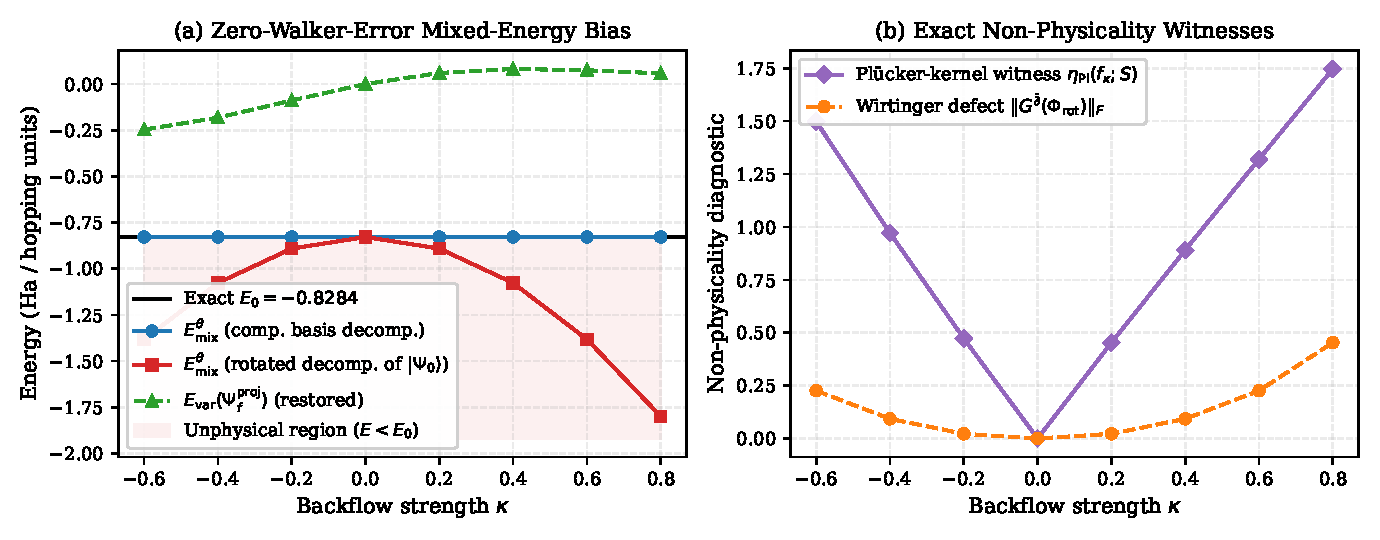
\includegraphics[width=\textwidth]{figures/fig1_backflow_bias_plucker.pdf}
\caption{Experiment 1 ($N=4, \eta=2$ Hubbard, $E_0 = -0.8284$). (a) Exact zero-walker-error mixed energy on computational-basis vs.\ rotated decompositions of $\ket{\Psi_0}$, alongside restored variational energy $E_{\mathrm{var}}(\Psi_f^{\mathrm{proj}})$. (b) Sharp Pl\"ucker-kernel witness $\eta_{\mathrm{Pl}}$ and Wirtinger defect $\|G^{\bar{\partial}}\|_F$.}
\label{fig:exp1}
\end{figure}

\paragraph{Experiment 2: Adversarial 10,000-trial audit of Theorem~\ref{thm:boost}.}
Across $10{,}000$ random complex Hermitian Hamiltonians ($d \in [2,13]$) and random complex unit state pairs $(\ket{\Psi_{\mathrm{sur}}}, \ket{\Psi_T})$, inequality \eqref{eq:boost} had \textbf{$0/10{,}000$ violations} (minimum slack $E_{\mathrm{cert}} - E_0 = 2.58\times 10^{-4}$, median boost $0.1504$, max boost $3.3951$). On the sharp boundary witness $H = \operatorname{diag}(-1,1)$, $\ket{\Psi_{\mathrm{sur}}} = (\cos 0.4, \sin 0.4)^\top$, $\ket{\Psi_T} = (1,0)^\top$ ($\mathcal{S} = \operatorname{span}\{\ket{\Psi_0}, \ket{\Psi_{\max}}\}$), $E_{\mathrm{sur}} = -0.696707$ boosts to $E_{\mathrm{cert}} = -1.000000000000 = E_0$ (gap $0.00$).

\paragraph{Experiment 3: 4-site Hubbard Block Hausdorff energy and oracle-free spectral-gap certificates.}
On the 4-site 1D Hubbard chain at half-filling ($8$ spin-orbitals, $D = 36$, $t=1, U=4$, $E_0 = -1.953145$, $E_1 = -1.412899$), Gershgorin's theorem gives the oracle-free enclosure $[-6, 14]$. Anchoring to the classical RHF determinant $\ket{\Psi_{\mathrm{sur}}}$ ($E_{\mathrm{sur}} = -0.472136$, overlap fidelity $0.7160$) and an imaginary-time correlated quantum trial $\ket{\Psi_T} \propto e^{-0.6 H}\ket{\Psi_{\mathrm{sur}}}$ ($E_T = -1.943285$, $b_0 = 0.8678$), Table~\ref{tab:exp3} and Figure~\ref{fig:exp2} report \emph{exact-$\Q$-verified} Block Hausdorff upper bounds on $E_0$ (with explicit rational classical-moment enclosure $\varepsilon_{a,k} = 10^{-10}$ for $k \ge 1$, absorbing double-precision evaluation and rational quantization) and \emph{oracle-free} two-edge visible spectral-gap certificates.
At $d=0$, using \emph{only} $(a_0, a_1)$ and linear cross-moments $(b_0, b_1)$ (zero $c_k$ measurements), Theorem~\ref{thm:boost}/Theorem~\ref{thm:hausdorff} certifies $E_0 \le -0.8708$ ($\varepsilon_b = 0$), $-0.8311$ ($\varepsilon_b = 0.002$), and $-0.7746$ ($\varepsilon_b = 0.005$), improving on RHF by $+0.399$, $+0.359$, and $+0.303$. At $d=1, \varepsilon_b=0.002$, the anchored certificate reaches $E_0 \le -1.7137$, strictly beating classical Krylov ($-1.6595$) by $+0.0542$ even under noisy linear shadows; at $d=2, \varepsilon_b=0$, it reaches $E_0 \le -1.9482$ (within $0.0049$ of exact $E_0$). With adaptive rational PSD shifts, at $d=2$ and $\varepsilon_b \ge 0.002$ the exact-$\Q$ anchored bound tightly tracks the floating-point classical Krylov floor ($-1.918107$ vs.\ $-1.918123$, quantization slack $1.6\times 10^{-5}$) and is strictly monotone in $\varepsilon_b$.
For the \emph{oracle-free} two-edge gap localizer ($d=2, K=6$), we plug $\theta_2 := \theta_{\mathrm{cert}} = 67936019/85356906 \approx 0.795905$ ($E_{\mathrm{cert}} = -1.918107$) directly from the exported single-edge certificate \texttt{hubbard4\_edge\_d2\_eps002.cert.json} (which already proves $\lambda_0 > \theta_2$ without knowing $E_0$). The dominant excited singlet visible to $\ket{\Psi_{\mathrm{sur}}}$ sits at $E_8 = +1.9110$ (weight $0.1528$; level~3 at $-0.5954$ carries weight $0.0033$). At $\varepsilon_b = 0.002$, exact rational certificates refute $[0, \theta_1] \cup [\theta_2, 1]$ down to $E_{\mathrm{cut}} = +3.00$ (exact-$\Q$ margin $-1.11\times 10^{-6}$, exported in \texttt{hubbard4\_gap\_d2\_E30\_eps002.cert.json}; at $\varepsilon_b = 0$, margin $-2.68\times 10^{-5}$), certifying an excited state strictly inside $(-1.9181, +3.00)$ without any oracle, and cleanly failing to reject for $E_{\mathrm{cut}} \le +2.50$.

\begin{table}[t]
\centering
\caption{Experiment 3: 4-site Hubbard chain ($D=36$, $E_0 = -1.953145$, RHF $E_{\mathrm{sur}} = -0.472136$). Every Anchored $(a,b)$ and Full $(a,b,c)$ bound is independently verified in exact rational arithmetic ($\Q$) via symmetry-checked pivoted $LDL^\top$ with explicit enclosure $\varepsilon_{a,k} = 10^{-10}$ ($k \ge 1$).}
\label{tab:exp3}
\small
\begin{tabular}{ccrrrr}
\toprule
$\varepsilon_b$ & Degree $d$ & Classical Krylov $(a)$ & Anchored $(a,b\text{ only})$ & Full $(a,b,c)$ & Exact-$\Q$ margin $(a,b)$ \\
\midrule
$0.000$ & $0$ & $-0.472136$ & $-0.870796$ & $-1.948452$ & $-4.31\times 10^{-8}$ \\
$0.000$ & $1$ & $-1.659517$ & $-1.906745$ & $-1.952736$ & $-1.78\times 10^{-9}$ \\
$0.000$ & $2$ & $-1.918123$ & $-1.948226$ & $-1.952929$ & $-7.74\times 10^{-10}$ \\
\midrule
$0.002$ & $0$ & $-0.472136$ & $-0.831127$ & $-1.903284$ & $-4.60\times 10^{-8}$ \\
$0.002$ & $1$ & $-1.659517$ & $-1.713670$ & $-1.924538$ & $-2.38\times 10^{-9}$ \\
$0.002$ & $2$ & $-1.918123$ & $-1.918107$ & $-1.928063$ & $-3.20\times 10^{-9}$ \\
\midrule
$0.005$ & $0$ & $-0.472136$ & $-0.774643$ & $-1.843284$ & $-3.97\times 10^{-8}$ \\
$0.005$ & $1$ & $-1.659517$ & $-1.659516$ & $-1.892758$ & $-1.48\times 10^{-9}$ \\
$0.005$ & $2$ & $-1.918123$ & $-1.918107$ & $-1.918120$ & $-3.20\times 10^{-9}$ \\
\midrule
$0.020$ & $0$ & $-0.472136$ & $-0.555073$ & $-1.543283$ & $-3.66\times 10^{-8}$ \\
$0.020$ & $2$ & $-1.918123$ & $-1.918091$ & $-1.918104$ & $-7.58\times 10^{-9}$ \\
\bottomrule
\end{tabular}
\end{table}

\begin{figure}[t]
\centering
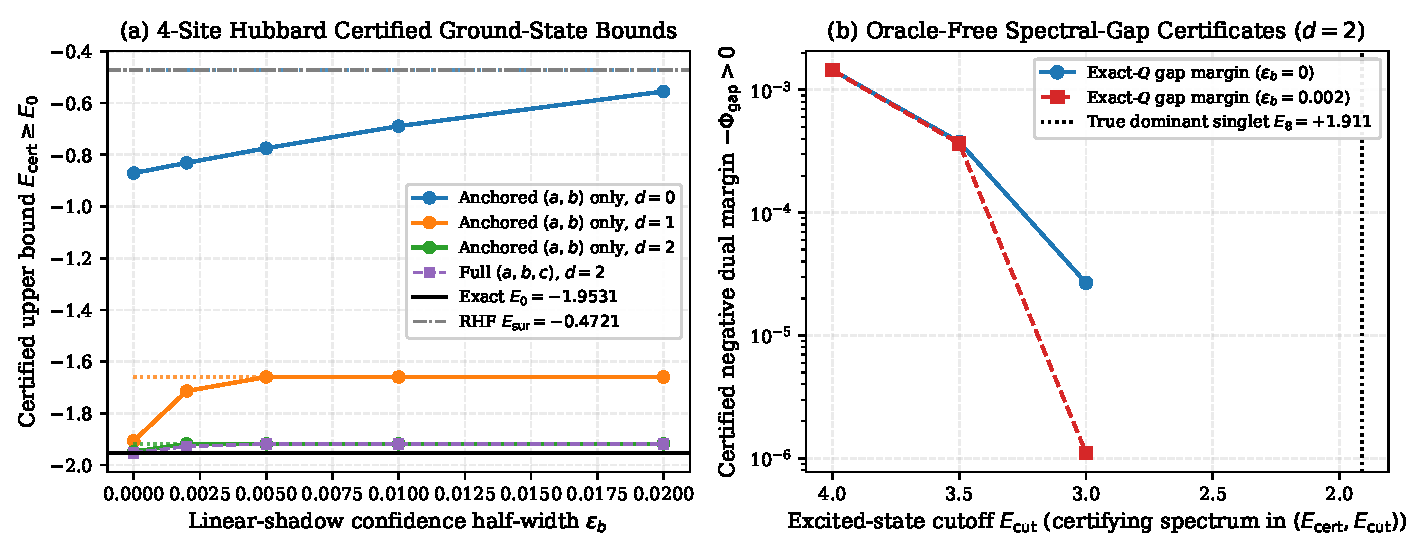
\includegraphics[width=\textwidth]{figures/fig2_hubbard_energy_gap_bounds.pdf}
\caption{Experiment 3 (4-site Hubbard, $D=36$). (a) Exact-$\Q$-verified ground-state upper bounds vs.\ linear-shadow confidence half-width $\varepsilon_b$ (dotted lines: classical Krylov). (b) Oracle-free exact-$\Q$ two-edge spectral-gap dual margins $-\Phi_{\mathrm{gap}}$ using $\theta_2 = \theta_{\mathrm{cert}} = 0.7959$ ($E_{\mathrm{cert}} = -1.9181$), certifying an excited state strictly inside $(-1.9181, E_{\mathrm{cut}})$.}
\label{fig:exp2}
\end{figure}

\paragraph{Experiment 4: Authentic Born-rule shadow coverage and Backflow-NQS PPI debiasing.}
All three parts of Experiment~4 simulate exact Born-rule global Haar shadows on $\C\ket{0} \oplus \mathcal{H}_D$ via Mezzadri QR sampling (zero synthetic Gaussian noise proxies):
(i) On the 4-site Hubbard chain ($D=36$, $20{,}000$ shots), empirical single-shot variances $[2.901, 1.570, 0.923, 0.564]$ for $k=0,1,2,3$ match the exact 3-design formula \eqref{eq:exact_3design_var} ($[2.904, 1.568, 0.921, 0.562]$) to three significant figures and sit cleanly below the universal complex bound $4 a_{2k}$ ($[4.000, 2.162, 1.271, 0.776]$, Figure~\ref{fig:exp3}a), while maximum single-shot magnitudes $[10.19, 7.49, 5.86, 4.62]$ obey $(D+2)\sqrt{a_{2k}}$.
(ii) Across $100$ independent 2-site Hubbard campaigns ($C = 31{,}000$ Born-rule shots/trial, $B=31$ MoM blocks, $\alpha = 0.05$, using universal $\sigma_k^2 = 4 a_{2k}$), the MoM box achieved \textbf{$100/100$ empirical coverage} ($\ge 95\%$ target) and \textbf{$100/100$ valid exact-$\Q$ energy certificates} ($E_{\mathrm{cert}} \ge E_0$). At this modest $C=31{,}000$ shot budget, conservative MoM radii safely fall back to $E_{\mathrm{sur}}$ ($0/100$ false improvements), illustrating fail-closed behavior; crossing into strict RHF improvement requires $\varepsilon_b \lesssim 0.02$ (corresponding to Willow-scale $10^5$--$10^6$ shots \cite[Table~S1.1]{jiang2026machine}).
(iii) On the 2-site Hubbard model ($D=6$), we generate $M=4{,}000$ gauge-aligned rotated complex Slater-determinant walkers $\{\Phi_a\}$ with purely classical RHF-based weights $g_a = 1 + 2|\operatorname{Re}\braket{\Psi_{\mathrm{RHF}}}{\phi(\Phi_a)}|$ and evaluate a biased non-holomorphic Backflow NQS ($0.88$ shrinkage plus $\kappa=0.5$ backflow residual from Experiment~1; surrogate-only bias $-0.0868$ on $h_{\mathrm{true}} = 0.7050$). Across $250$ trials sampling $m_{\mathrm{cal}}=80$ walkers i.i.d.\ with replacement and measuring each calibration draw with $C_{\mathrm{cal}} = 256$ independent Born-rule Haar shadows ($5{,}120{,}000$ total Born-rule shots), $\widehat{h}^{\mathrm{PPI}}$ eliminates bias ($-0.00139$), achieves a \textbf{$7.40\times$ variance reduction} over raw Born-rule shadow subsampling ($\mathrm{RMSE}=0.0257$ vs.\ $0.0701$), yields an \textbf{$11.42\times$ MSE reduction} over the biased Backflow NQS alone, and closely tracks the theoretical Proposition~\ref{prop:ppi}(ii) variance ($6.61\times 10^{-4}$ empirical vs.\ $5.79\times 10^{-4}$ theoretical; Figure~\ref{fig:exp3}b).

\begin{figure}[t]
\centering
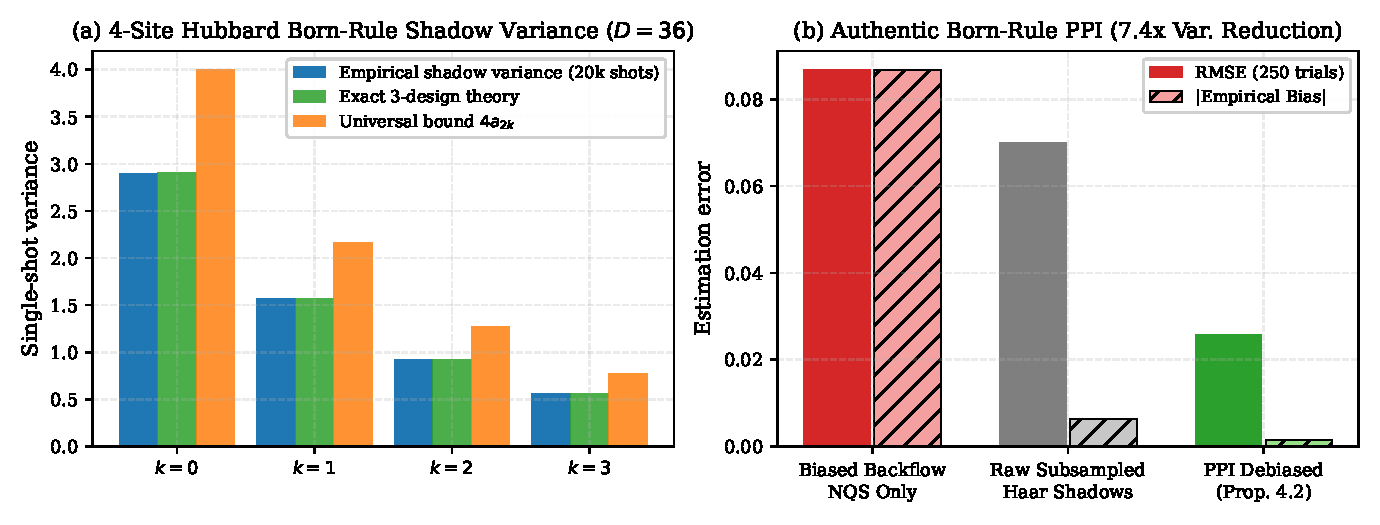
\includegraphics[width=\textwidth]{figures/fig3_finite_sample_coverage_ppi.pdf}
\caption{Experiment 4 (100\% authentic Born-rule global Haar shadows). (a) Empirical single-shot variance vs.\ exact 3-design theory and universal bound $4 a_{2k}$ on 4-site Hubbard ($D=36$, 20,000 shots). (b) Authentic Backflow-NQS PPI debiasing on 2-site Hubbard across 250 trials ($5.12\times 10^6$ Born-rule shots; $7.40\times$ variance reduction over raw shadows, $11.42\times$ MSE reduction over biased NQS).}
\label{fig:exp3}
\end{figure}

\section{Formal Verification Manifest and Reproducibility}

To satisfy AIRR Gate~2 and Lean~4 Level~L2 verification with strict specification transparency, \texttt{lean/QcQmcCert.lean} (pinned to \texttt{leanprover/lean4:v4.35.0} with zero external dependencies) formally proves the algebraic, complex-vector orthogonal projection, $2\times 2$ variational-boost, and complex spectral-measure conic-dual soundness cores over an arbitrary linearly ordered commutative field \texttt{OrdField K} (covering $\R$ and $\Q$, with complex numbers represented explicitly via \texttt{ComplexK K}). It builds cleanly via \texttt{lake build} in $2.0\,\mathrm{s}$ with zero \texttt{sorry} and zero warnings. Table~\ref{tab:manifest} maps each Lean~4 theorem to its exact formalized scope and audited axioms (via \texttt{lean/AuditAxioms.lean}); none require even \texttt{Classical.choice}. Complex-analytic Grassmannian chart arguments (Theorem~\ref{thm:holo}), Weingarten 3-design moments \eqref{eq:exact_3design_var}, and Chebyshev/Hoeffding probability tails (Proposition~\ref{prop:ppi}) are proved analytically in prose. All five exact rational dual certificates in \texttt{results/rational\_certificates/} and all file digests in \texttt{SHA256SUMS.json} are publicly archived at \url{https://github.com/lluiseriksson/qcqmc-spectral-certificates} and replayed in one command via \texttt{python scripts/verify\_all.py}.

\begin{table}[t]
\centering
\caption{Auditable Claim-to-Theorem Manifest (\texttt{lean/QcQmcCert.lean}, Lean~v4.35.0, 0 \texttt{sorry}, 0 warnings).}
\label{tab:manifest}
\scriptsize
\setlength{\tabcolsep}{4pt}
\begin{tabular}{@{}p{2.1cm}p{5.5cm}p{5.2cm}p{2.2cm}@{}}
\toprule
Result & Lean 4 Symbol (\texttt{QcQmcCert.*}) & Exact Formalized Scope & Audited Axioms \\
\midrule
Remark~\ref{rem:collapse} & \texttt{linear\_projector\_collapse} & Left-projector $G_0 + PA$ collapse & none \\
Theorem~\ref{thm:plucker} & \texttt{plucker\_kernel\_distance\_min}, \texttt{\_attained}, \texttt{\_min\_complex} & Real \& \texttt{ComplexK} projection floor $\|g - v\|^2 \ge \|g_\perp\|^2$ & \texttt{propext}, \texttt{Quot.sound} \\
Theorem~\ref{thm:bias} & \texttt{mixed\_estimator\_bias\_decomp}, \texttt{holomorphic\_zero\_bias}, \texttt{nonholomorphic\_bias\_persists} & Finite-walker algebraic bias split \& eigenstate residual persistence & \texttt{propext}, \texttt{Quot.sound} \\
Theorem~\ref{thm:boost} & \texttt{variational\_boost\_spectral\_bound}, \texttt{\_hamiltonian}, \texttt{\_sharp} & $2\times 2$ PSD spectral-edge bound, Hamiltonian form, rank-1 identity & none \\
Theorem~\ref{thm:hausdorff}(i) & \texttt{block\_hausdorff\_edge\_soundness}, \texttt{\_edge\_soundness\_complex} & Real \& \texttt{ComplexK} spectral-measure single-edge dual soundness & \texttt{propext}, \texttt{Quot.sound} \\
Theorem~\ref{thm:hausdorff}(ii) & \texttt{block\_hausdorff\_gap\_soundness}, \texttt{\_gap\_soundness\_complex} & Real \& \texttt{ComplexK} spectral-measure two-edge gap dual soundness & \texttt{propext}, \texttt{Quot.sound} \\
Theorem~\ref{thm:hausdorff} & \texttt{linear\_box\_upper\_bound} & Box transfer over $|b - \hat{b}| \le \varepsilon$, $c \in [0,1]$ & none \\
Prop.~\ref{prop:ppi}(ii) & \texttt{ppi\_control\_variate\_unbiased} & Finite-population expectation identity (algebraic core) & \texttt{propext}, \texttt{Quot.sound} \\
\bottomrule
\end{tabular}
\end{table}

\section{Limitations and Continuation Frontier}

We highlight four concrete limitations that define immediate next steps: (1) Theorem~\ref{thm:holo} (complex Grassmannian holomorphicity) and the probabilistic tails/Weingarten moments of Section~4.1 are proved analytically in prose while Lean~4 formalizes the algebraic, complex-projection, variational-boost, and complex conic-dual core; formalizing the complex-analytic Grassmannian chart proof in Mathlib is left to future work. (2) At higher polynomial degree ($d \ge 3$), monomial Hankel bases become increasingly ill-conditioned under exact rational $LDL^\top$ certification (though adaptive shifts already reduce our $d=2$ slack to $1.6\times 10^{-5}$ on 4-site Hubbard); switching to Chebyshev-basis localizers $T_k(T)$ should reduce condition numbers exponentially for high-degree rational bounds. (3) Conservative Median-of-Means constants require large shot counts ($10^5$--$10^6$) to beat strong classical baselines; integrating sharp Empirical-Bernstein / Catoni bounds with matchgate shadow variance estimators is a high-leverage practical extension. (4) Two-edge gap certification detects excited states visible to $\operatorname{span}\{\ket{\Psi_{\mathrm{sur}}}, \ket{\Psi_T}\}$ and cannot exclude symmetry sectors strictly orthogonal to both states.

\bibliographystyle{plain}
\bibliography{references}
\end{document}
